\section{Stacked Capsule Autoencoders (\textsc{scae})}
\label{sec:caps_decoders}
Segmenting an image into parts is non-trivial, so we begin by abstracting away pixels and the part-discovery stage, and develop the \gls{CCAu} (\Cref{sec:constellation}).
It uses two-dimensional points as parts, and their coordinates are given as the input to the system. \Gls{CCAu} learns to model sets of points as arrangements of familiar constellations, each of which has been transformed by an independent similarity transform. The \gls{CCAu} learns to assign individual points to their respective constellations—without knowing the number of constellations or their individual shapes in advance.  Next, in Section 2.2, we develop the \glsreset{PCAu}\gls{PCAu} which learns to infer parts and their poses from images. Finally, we stack the \glsreset{OCAu}\gls{OCAu}, which closely resembles the \gls{CCAu}, on top of the \gls{PCAu} to form the \glsreset{SCAu}\gls{SCAu}.



\subsection{Constellation Autoencoder (\textsc{ccae})}
\label{sec:constellation}

Let $\set{\bx_m\mid m=1,\dots,M}$ be a set of two-dimensional input points, where every point belongs to a constellation as in \Cref{fig:constellations}.
We first encode all input points (which take the role of part capsules) with Set Transformer \citep{Lee2019set}---a permutation-invariant encoder $h^\mathrm{caps}$ based on attention mechanisms---into $K$ object capsules.
An object capsule $k$ consists of a capsule feature vector $\bc_k$, its presence probability $a_k \in \interval{0, 1}$ and a $3 \times 3$ \glsreset{OV}\gls{OV} matrix, which represents the affine transformation between the object (constellation) and the viewer.
Note that each object capsule can represent only one object at a time.
Every object capsule uses a separate \gls{MLP} $\operatorname{h_k^\mathrm{part}}$ to predict $N \leq M$ part candidates from the capsule feature vector $\bc_k$.
Each candidate consists of the conditional probability $a_{k,n} \in \interval{0, 1}$ that a given candidate part exists, an associated scalar standard deviation $\lambda_{k,n}$, and a $3 \times 3$ \glsreset{OP}\gls{OP} matrix, which represents the affine transformation between the object capsule and the candidate part\footnote{Deriving these matrices from the capsule feature vector allows for deformable objects. We model \gls{OP}s as the sum of an input-dependent component and a constant bias. We encourage different capsules to specialize to different constellations by putting a strong $L_2$ penalty on the former.}.
Candidate predictions $\mu_{k,n}$ are given by the product of the object capsule \gls{OV} and the candidate \gls{OP} matrices.
We then model each input part as a Gaussian mixture, where $\mu_{k,n}$ and $\lambda_{k,n}$ are the centers and standard deviations of the isotropic components.
See \Cref{fig:capsule_arch,fig:sca_arch} for illustration; formal description follows:
\begin{align}
    &\textsc{ov}_{1:K}, \bc_{1:K}, a_{1:K} = \operatorname{h^\mathrm{caps}} (\bx_{1:M}) &\text{encode object capsule parameters,}\\
    % 
    &\textsc{op}_{k,1:N}, a_{k, 1:N}, \lambda_{k, 1:N} = \operatorname{h_k^\mathrm{part}} (\bc_k) &\text{decode candidate parameters from $c_k$'s,}\\
    % 
    &V_{k,n} = \textsc{ov}_k \textsc{op}_{k,n} &\text{decode a part pose candidate,}\\
    % 
    &\p{\bx_m}{k,n} = \gauss{\bx_m \mid \mu_{k,n}, \lambda_{k,n}} &\text{turn candidates into mixture components,}\label{eq:component}
\end{align}
\begin{equation}
    \p{\bx_{1:M}} = \prod_{m=1}^M \sum_{k=1}^K \sum_{n=1}^{N}  
    \frac{a_k a_{k,n}}{\sum_i a_i \sum_j a_{i,j}}
    \,\p{\bx_m}{k,n}\,. \label{eq:constellation_likelihood}
\end{equation}
The model is trained without supervision by maximizing the likelihood of part capsules in \Cref{eq:constellation_likelihood} subject to sparsity constraints, \textit{cf}.\ \Cref{sec:losses}.
The part capsule $m$ can be assigned to the object capsule $k^\star$ as $k^\star = \operatorname{arg\,max}_{k}~a_k a_{k,n}\;\p{\bx_m}{k,n}$.\footnote{We treat parts as independent and evaluate their probability under the same mixture model. While there are no clear 1:1 connections between parts and predictions, it seems to work well in practice.}
\begin{figure} 
    \centering
    \begin{minipage}[c]{0.35\linewidth}
        \centering
        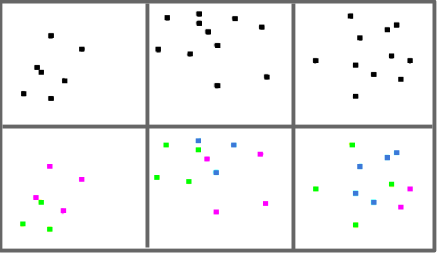
\includegraphics[width=\linewidth]{figures/SCA/consinvert5}
    \end{minipage}
    \hfill
    \begin{minipage}[c]{0.63\linewidth}
        \centering
        \caption{
            Unsupervised segmentation of points belonging to up to three constellations of squares and triangles at different positions, scales and orientations. 
            The model is trained to reconstruct the points (top row) under the \gls{CCAu} mixture model. The bottom row colors the points based on the parent with highest posterior probability in the mixture model. 
            The right-most column shows a failure case.
            Note that the model uses sets of points, not pixels, as its input; we use images  only to visualize the constellation arrangements.
        }
        \label{fig:constellations}
    \end{minipage}
\end{figure}
Empirical results show that this model is able to perform unsupervised instance-level segmentation of points belonging to different constellations, even in data which is difficult to interpret for humans. See \Cref{fig:constellations} for an example and \Cref{sec:constellation_expr} for details.

\subsection{Part Capsule Autoencoder (\textsc{pcae})}
\label{sec:img_capsule}
Explaining images as geometrical arrangements of parts requires first inferring what parts the images are composed of, as well as the relationships of the parts to the viewer (which we call their poses). For the \gls{CCAu} a part is just a 2D point, but here each part capsule has a six \gls{DOF} pose, a presence variable and a unique identity. We frame the part-discovery problem as auto-encoding: the encoder learns to infer the poses and presences of different part capsules, while the decoder learns an image template for each part (\cref{fig:learned_templates}) similar to \cite{Tieleman2014thesis,Eslami2016air}. The templates corresponding to present parts are affine-transformed using their poses, and the pixels of these transformed templates are used to create a separate mixture model for each image pixel.
The \gls{PCAu} is followed by an \glsreset{OCAu}\gls{OCAu}, which closely resambles the \gls{CCAu} and is described in \Cref{sec:ocae}.

Let $\by \in \interval{0, 1}^{h \times w \times c}$ be the image.
We limit the maximum number of part capsules to $M$ and use an encoder to infer their poses $\bx_m \in \RR^6$, presence probabilities $d_m \in \interval{0, 1}$, and special features $\bz_m \in \RR^{c_z}$, one per part capsule.
The latter do not take part in direct image reconstruction, but inform the \gls{OCAu} about special aspects of the corresponding part; they are trained by backpropagating derivatives from the \gls{OCAu}.

At present, we do not allow multiple occurrences of the same type of part in an image, so the part capsules themselves are not replicated across space, though they could be.
However, we do need to recognize the part wherever it occurs in the image, and therefore the encoder consists of a \gls{CNN} with a bottom-up attention mechanism; for every part capsule $k$, it predicts a feature map $\bf{e}_k$ of $6 \text{\,(pose)} + 1 \text{\,(presence)} + c_z \text{\,(special features)}$ capsule parameters with spatial dimensions $h_e \times w_e$\,, as well as a single-channel attention mask $\bf{a}_k$.
The final parameters for that capsule are computed as $\sum_{i} \sum_j \bf{e}_{k, i,j} \operatorname{softmax}(\bf{a})_{k,i,j}$, where $\operatorname{softmax}$ is along the spatial dimensions.
This is similar to global average pooling, but allows some spatial locations to contribute to the final result more than others; we call this approach \textit{attention-based pooling}. Its effect on the model performance is analyzed in \Cref{sec:ablation}.

The image pixels are modelled as independent Gaussian mixtures.
For every pixel, we take the corresponding pixels of the transformed templates and treat them as centers of isotropic Gaussian components with constant variance.
Their mixing probabilities are proportional to both presence probabilities of part capsules and a function $f_c: \RR^c \mapsto \interval{0, 1}$ of the color value at that location\footnote{
Templates are assumed to be sparse; if there exists a template that has a non-zero value at a given location, then this templates should be used.}, where $c$ is the number of image channels. 
More formally:
\begin{align}
    &\bx_{1:M}, d_{1:M}, \bz_{1:M} = \operatorname{h^{\mathrm{enc}}}(\by) &\text{encode the image to part capsule parameters,}\\
    &\widehat{T}_m = \operatorname{TransformImage} (T_m, \bx_m)  &\text{apply affine transforms to image templates,}\\
    % 
    &p^y_{m,i,j} \propto d_m \operatorname{f_c}\left(\widehat{T}_{m,i,j}\right) &\text{compute mixing probabilities,}\\
    % 
    &\p{\by} = \prod_{i,j} \sum_{m=1}^M p^y_{m,i,j}\, \gauss{y_{i,j} \mid \widehat{T}_{m,i,j}, \sigma^2_y} &\text{calculate image likelihood.} \label{eq:im_likelihood}
\end{align}

\subsection{Object Capsule Autoencoder (\textsc{ocae})}
\label{sec:ocae}
% \todo{\ak{explain why constellation and object aes are differnet}}

The next step is to find objects in the already discovered parts\footnote{
    Discovered objects are {\it not} used top-down to refine the presences or poses of the parts during inference. However, the derivatives backpropagated via \gls{OCAu} refine the lower-level encoder network that infers the parts.
}.
To do so, we use concatenated poses $\bx_m$, special features $\bz_m$ and flattened templates $T_m$ (which convey the identity of the part capsule)
as an input to the \gls{OCAu}, which differs from the \gls{CCAu} in the following ways.
Firstly, we feed part capsule presence probabilities $d_m$ into the \gls{OCAu}'s encoder---these are used to bias the Set Transformer's attention mechanism to not take absent points into account.
% ; see \Cref{app:set_transformer} for details.
Secondly, $d_m$'s are also used to weigh the part-capsules' log-likelihood, \textit{cf}. \Cref{eq:constellation_likelihood}.
Additionally, we stop the gradient on all of \gls{OCAu}'s inputs except the special features to improve training stability and avoid the problem of collapsing latent variables; see\eg \cite{Rasmus2015ladder}.
Finally, parts discovered by the \gls{PCAu} have independent identities (templates and special features rather than 2D points).
Therefore, every part-pose is explained as an independent mixture of predictions from object-capsules---where every object capsule makes exactly $M$ candidate predictions $V_{k,1:M}$, or exactly {\bf one} candidate prediction per part.
Consequently, the part-capsule likelihood is given by,
\begin{equation}
    \p{\bx_{1:M}, d_{1:M}} = \prod_{m=1}^M \left[\, \sum_{k=1}^K  
    \frac{a_k a_{k,m}}{\sum_i a_i \sum_j a_{i,j}}
    \,\p{\bx_m}{k,m}\right]^{d_m}\,. \label{eq:mod_constellation_likelihood}
\end{equation}

\begin{figure}
    \centering
    \begin{minipage}[b]{.47\linewidth}
    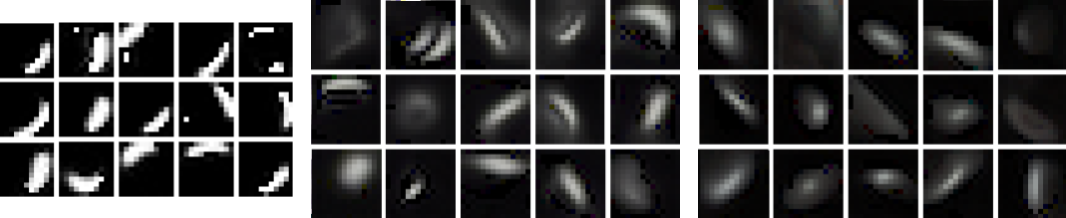
\includegraphics[width=\linewidth]{figures/SCA/templates}
    \end{minipage}
    \hfill
    \begin{minipage}[b]{.52\linewidth}
    \caption{Templates learned on \textsc{mnist} (left) as well as sobel-filtered \textsc{svhn} (middle) and \textsc{cifar10} (right). In each case templates converge to strokes. For \textsc{svhn} they often take the form of double strokes---this is due to sobel filtering, which effectively extracts edges.}
    \label{fig:learned_templates}
    \end{minipage}
\end{figure}
\begin{figure}
    \centering
    % 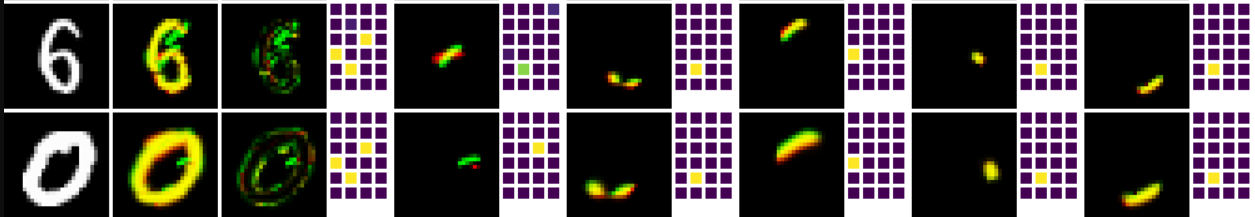
\includegraphics[width=\linewidth]{figures/SCA/mnist_rec}
    % 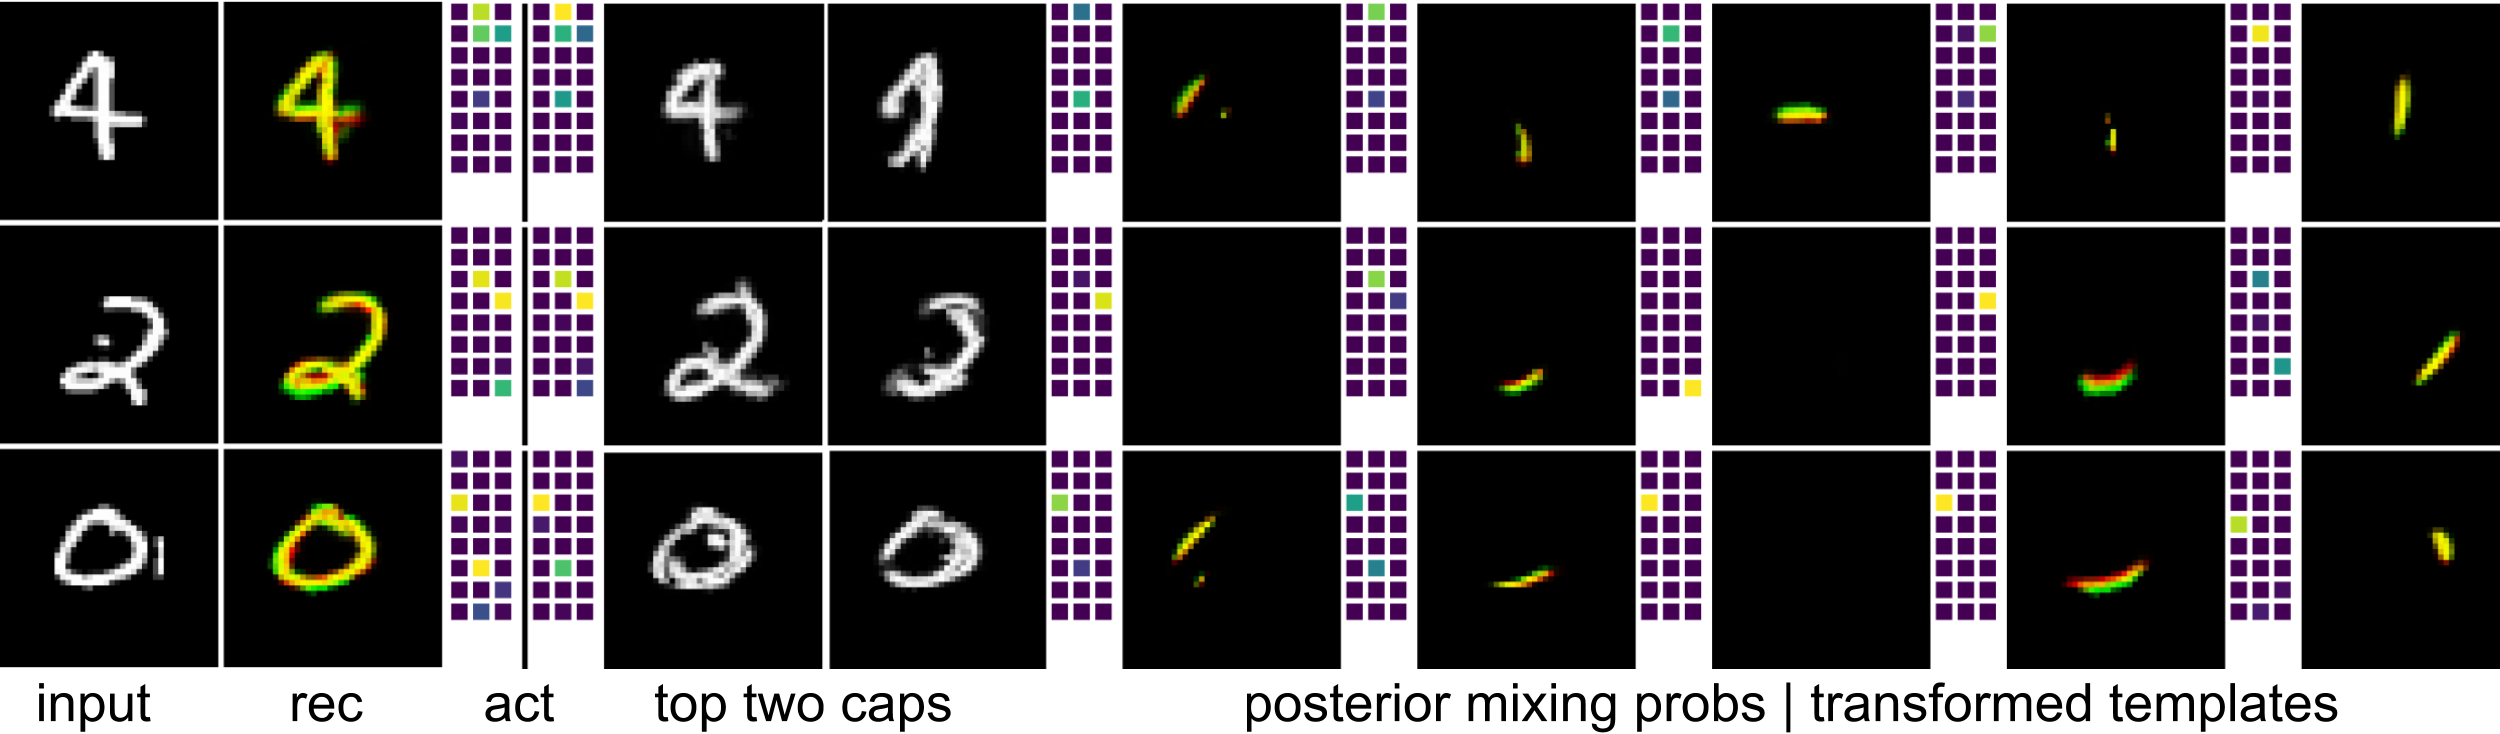
\includegraphics[width=.5\linewidth]{figures/SCA/mnist_strokes}
    \begin{subfigure}[c]{.045\linewidth}
        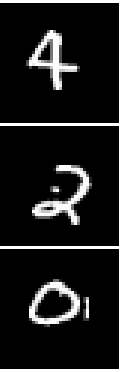
\includegraphics[width=\linewidth]{figures/SCA/mnist/inputs}
        \caption{}
    \end{subfigure}
    \hfill
    \begin{subfigure}[c]{.045\linewidth}
        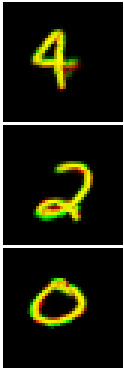
\includegraphics[width=\linewidth]{figures/SCA/mnist/recs}
        \caption{}
    \end{subfigure}
        \hfill
    \begin{subfigure}[c]{.0295\linewidth}
        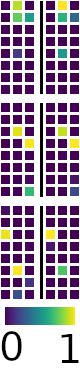
\includegraphics[width=\linewidth]{figures/SCA/mnist/acts}
        \caption{}
    \end{subfigure}
    \hfill
    \begin{subfigure}[c]{.09\linewidth}
        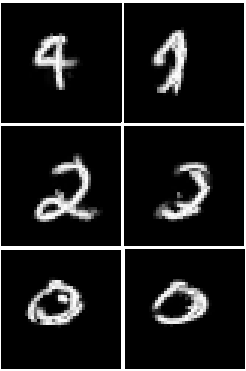
\includegraphics[width=\linewidth]{figures/SCA/mnist/caps_recs}
        \caption{}
    \end{subfigure}
    \hfill
    \begin{subfigure}[c]{.225\linewidth}
        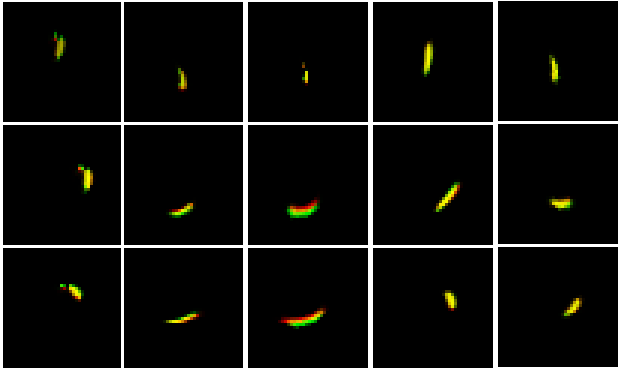
\includegraphics[width=\linewidth]{figures/SCA/mnist/transformed_templates}
        \caption{}
    \end{subfigure}
    \hfill
    \begin{minipage}[c]{.52\linewidth}
        \caption{
        $40\times40$ \textsc{mnist} (a) images and their (b) reconstructions from part capsules in red and object capsules in green, with overlapping regions in yellow.
        Only a few object capsules are activated for every input (c) a priori (left) and even fewer are needed to reconstruct it (right).
        The most active capsules (d) capture object identity and the majority of information about its appearance. 
        Finally, (e) affine-transformed templates show how exactly parts are used to reconstruct the images.
        }
        \label{fig:mnist_rec}
    \end{minipage}
\end{figure}
\subsection{Achieving Sparse and Diverse Capsule Presences}
\label{sec:losses}
Stacked Capsule Autoencoders are trained to maximise pixel and part log-likelihoods ($\loss[\mathrm{ll}]{} = \log\p{\by} + \log\p{\bx_{1:M}}$).
If not constrained, however, they tend to either use all of the part and object capsules to explain every data example, or collapse onto using always the same subset of capsules, regardless of the input.
We would like the model to use different sets of part-capsules for different input examples and to specialize object-capsules to particular arrangements of parts; to encourage this, we impose sparsity and entropy constraints.  We evaluate their importance in \Cref{sec:ablation}.

We first define prior and posterior object-capsule presence as follows.
For a minibatch of size {\small$B$} with {\small$K$} object capsules and $M$ part capsules we define a minibatch of prior capsule presence $a^\mathrm{prior}_{1:K}$ with dimension {\small$[B, K]$} and posterior capsule presence $a^\mathrm{posterior}_{1:K,1:M}$ with dimension {\small$[B, K, M]$} as,
\begin{equation}
    a^\mathrm{prior}_k = a_k \max_m a_{m,k}\,,
    \qquad
    a^\mathrm{posterior}_{k,m} = a_k a_{k,m}\;\gauss{\bx_m \mid m,k}\,,
\end{equation}
respectively; the former is the maximum presence probability among predictions from object capsule $k$ while the latter is the unnormalized mixing probability used to explain part capsule~$m$.
\begin{description}[leftmargin=\parindent]
\item[Prior sparsity]
    Let $\overline{u}_k = \frac{1}{B} \sum_{b=1}^B a^\mathrm{prior}_{b,k}$ the average presence probability of the object capsule $k$ among different training examples, and $\widehat{u}_b = \sum_{k=1}^K a^\mathrm{prior}_{b,k}$ the sum of object capsule presence probabilities for a given example.
    If we assume that training examples contain objects from different classes uniformly at random and we would like to assign the same number of object capsules to every class then each class would obtain $\nicefrac{K}{C}$ capsules.
    Moreover, if we assume that only one object is present in every image, then $\nicefrac{B}{C}$ object capsules should be present for every input example.
    To this end, we minimize,
    \begin{equation}
        \loss[\mathrm{prior}]{} = 
        \frac{1}{B} \sum_{b=1}^B ||\widehat{u}_b  - \frac{K}{C} ||_2
        +
         \frac{1}{K} \sum_{k=1}^K || \overline{u}_k  - \frac{B}{C} ||_2\,. \label{eq:prior_sparsity}
    \end{equation}
    % 
\item[Posterior Sparsity]
    Similarity, let $\overline{v}_k$ and $\widehat{v}_b$ be the the normalized versions of  $\sum_{k,m} a^\mathrm{posterior}_{b,k,m}$
    and $\sum_{b,m} a^\mathrm{posterior}_{b,k,m}$, respectively.
    We find it beneficial to minimize the within-example entropy of capsule posterior presence $\mathcal{H}(\overline{v}_k)$ and maximize its between-example entropy $\mathcal{H}(\widehat{v}_b)$, where $\mathcal{H}$ is the entropy \todo{\ak{say why it is beneficial}}. The final loss reads as,
    \begin{equation}
        \loss[\mathrm{posterior}]{} = \frac{1}{K} \sum_{k=1}^K \mathcal{H}(\overline{v}_k) - \frac{1}{B} \sum_{b=1}^B \mathcal{H}(\widehat{v}_b)\,. \label{eq:posterior_sparsity}
    \end{equation}
% 
\item[Every active object capsule should explain at least two parts]
    We say that an object capsule has `won' a part if it has the highest posterior mixing probability for that part among other object capsules.
    We then create binary labels for each of object capsules, where the label is $1$ if the capsule wins at least two parts and it is $0$ otherwise.
    The final loss takes the form of binary cross-entropy between the generated label and the prior capsule presence. This loss is used only for the stand-alone constellation model experiments on point data, \textit{cf}. \Cref{sec:constellation,sec:constellation_expr}.
% 
\end{description}
\begin{figure}
    \centering
    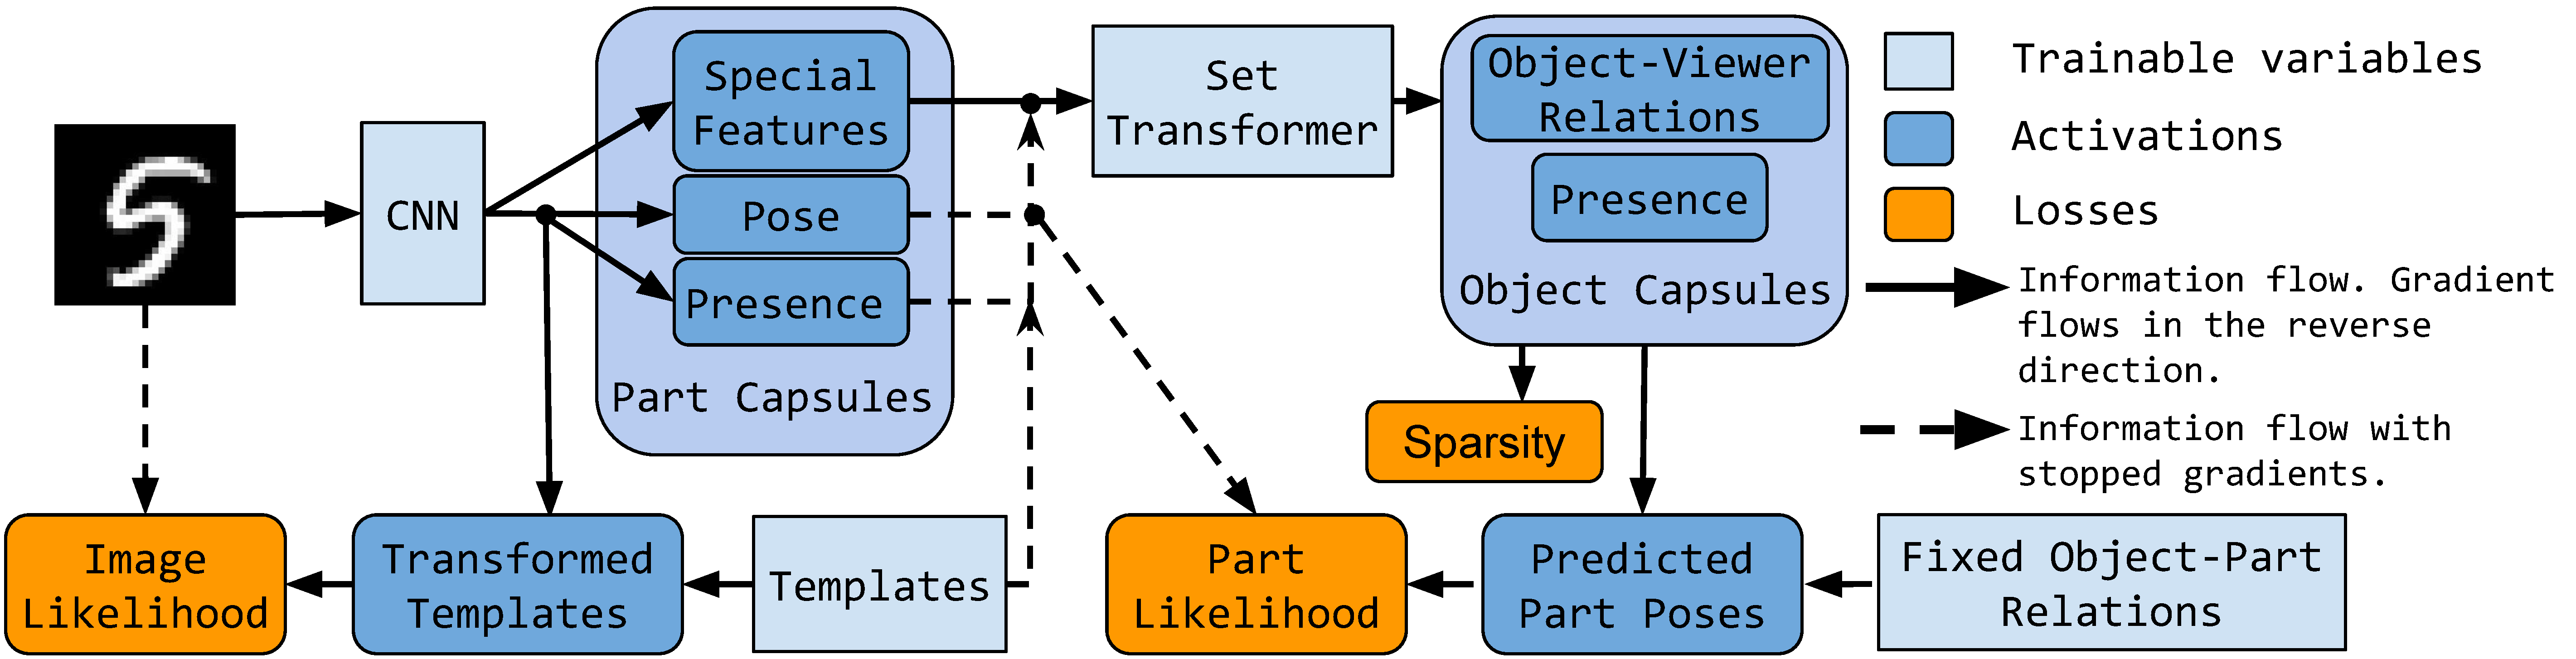
\includegraphics[width=\linewidth]{figures/SCA/sca_architecture_v3}
    \caption{\gls{SCAu} architecture.}
    \label{fig:sca_arch}
\end{figure}
\cref{fig:sca_arch} shows the schematic architecture of \gls{SCAu}. We optimize a weighted sum of image and part likelihoods and the auxiliary losses. 
Loss weight selection process as well as the values used for experiments are explained in \Cref{app:models}.

In order to make the values of presence probabilities ($a_k, a_{k,m}$ and $d_m$) closer to binary we inject uniform noise $\in \interval{-2, 2}$ into logits, similar to \cite{Tieleman2014thesis}.
This forces the model to predict logits that are far from zero to avoid stochasticity and makes the predicted presence probabilities close to binary.
Interestingly, it tends to work better in our case than using the Concrete distribution \citep{Maddison2017concrete}.